\documentclass[aspectratio=169]{beamer}

%Textos en español
\usepackage{babel}

% Document metadata
%\title{Programs}
%\subtitle{iHub-Data, IIIT Hyderabad}
%\author[TL]{Pilot Programs from IIIT Hyderabad}
%\institute{iHub-Data, IIIT Hyderabad}
%\date{\today}

% Imagen para la página del título (utilice la opción includegraphics para dimensionarla/ubicarla correctamente)
\titlegraphic{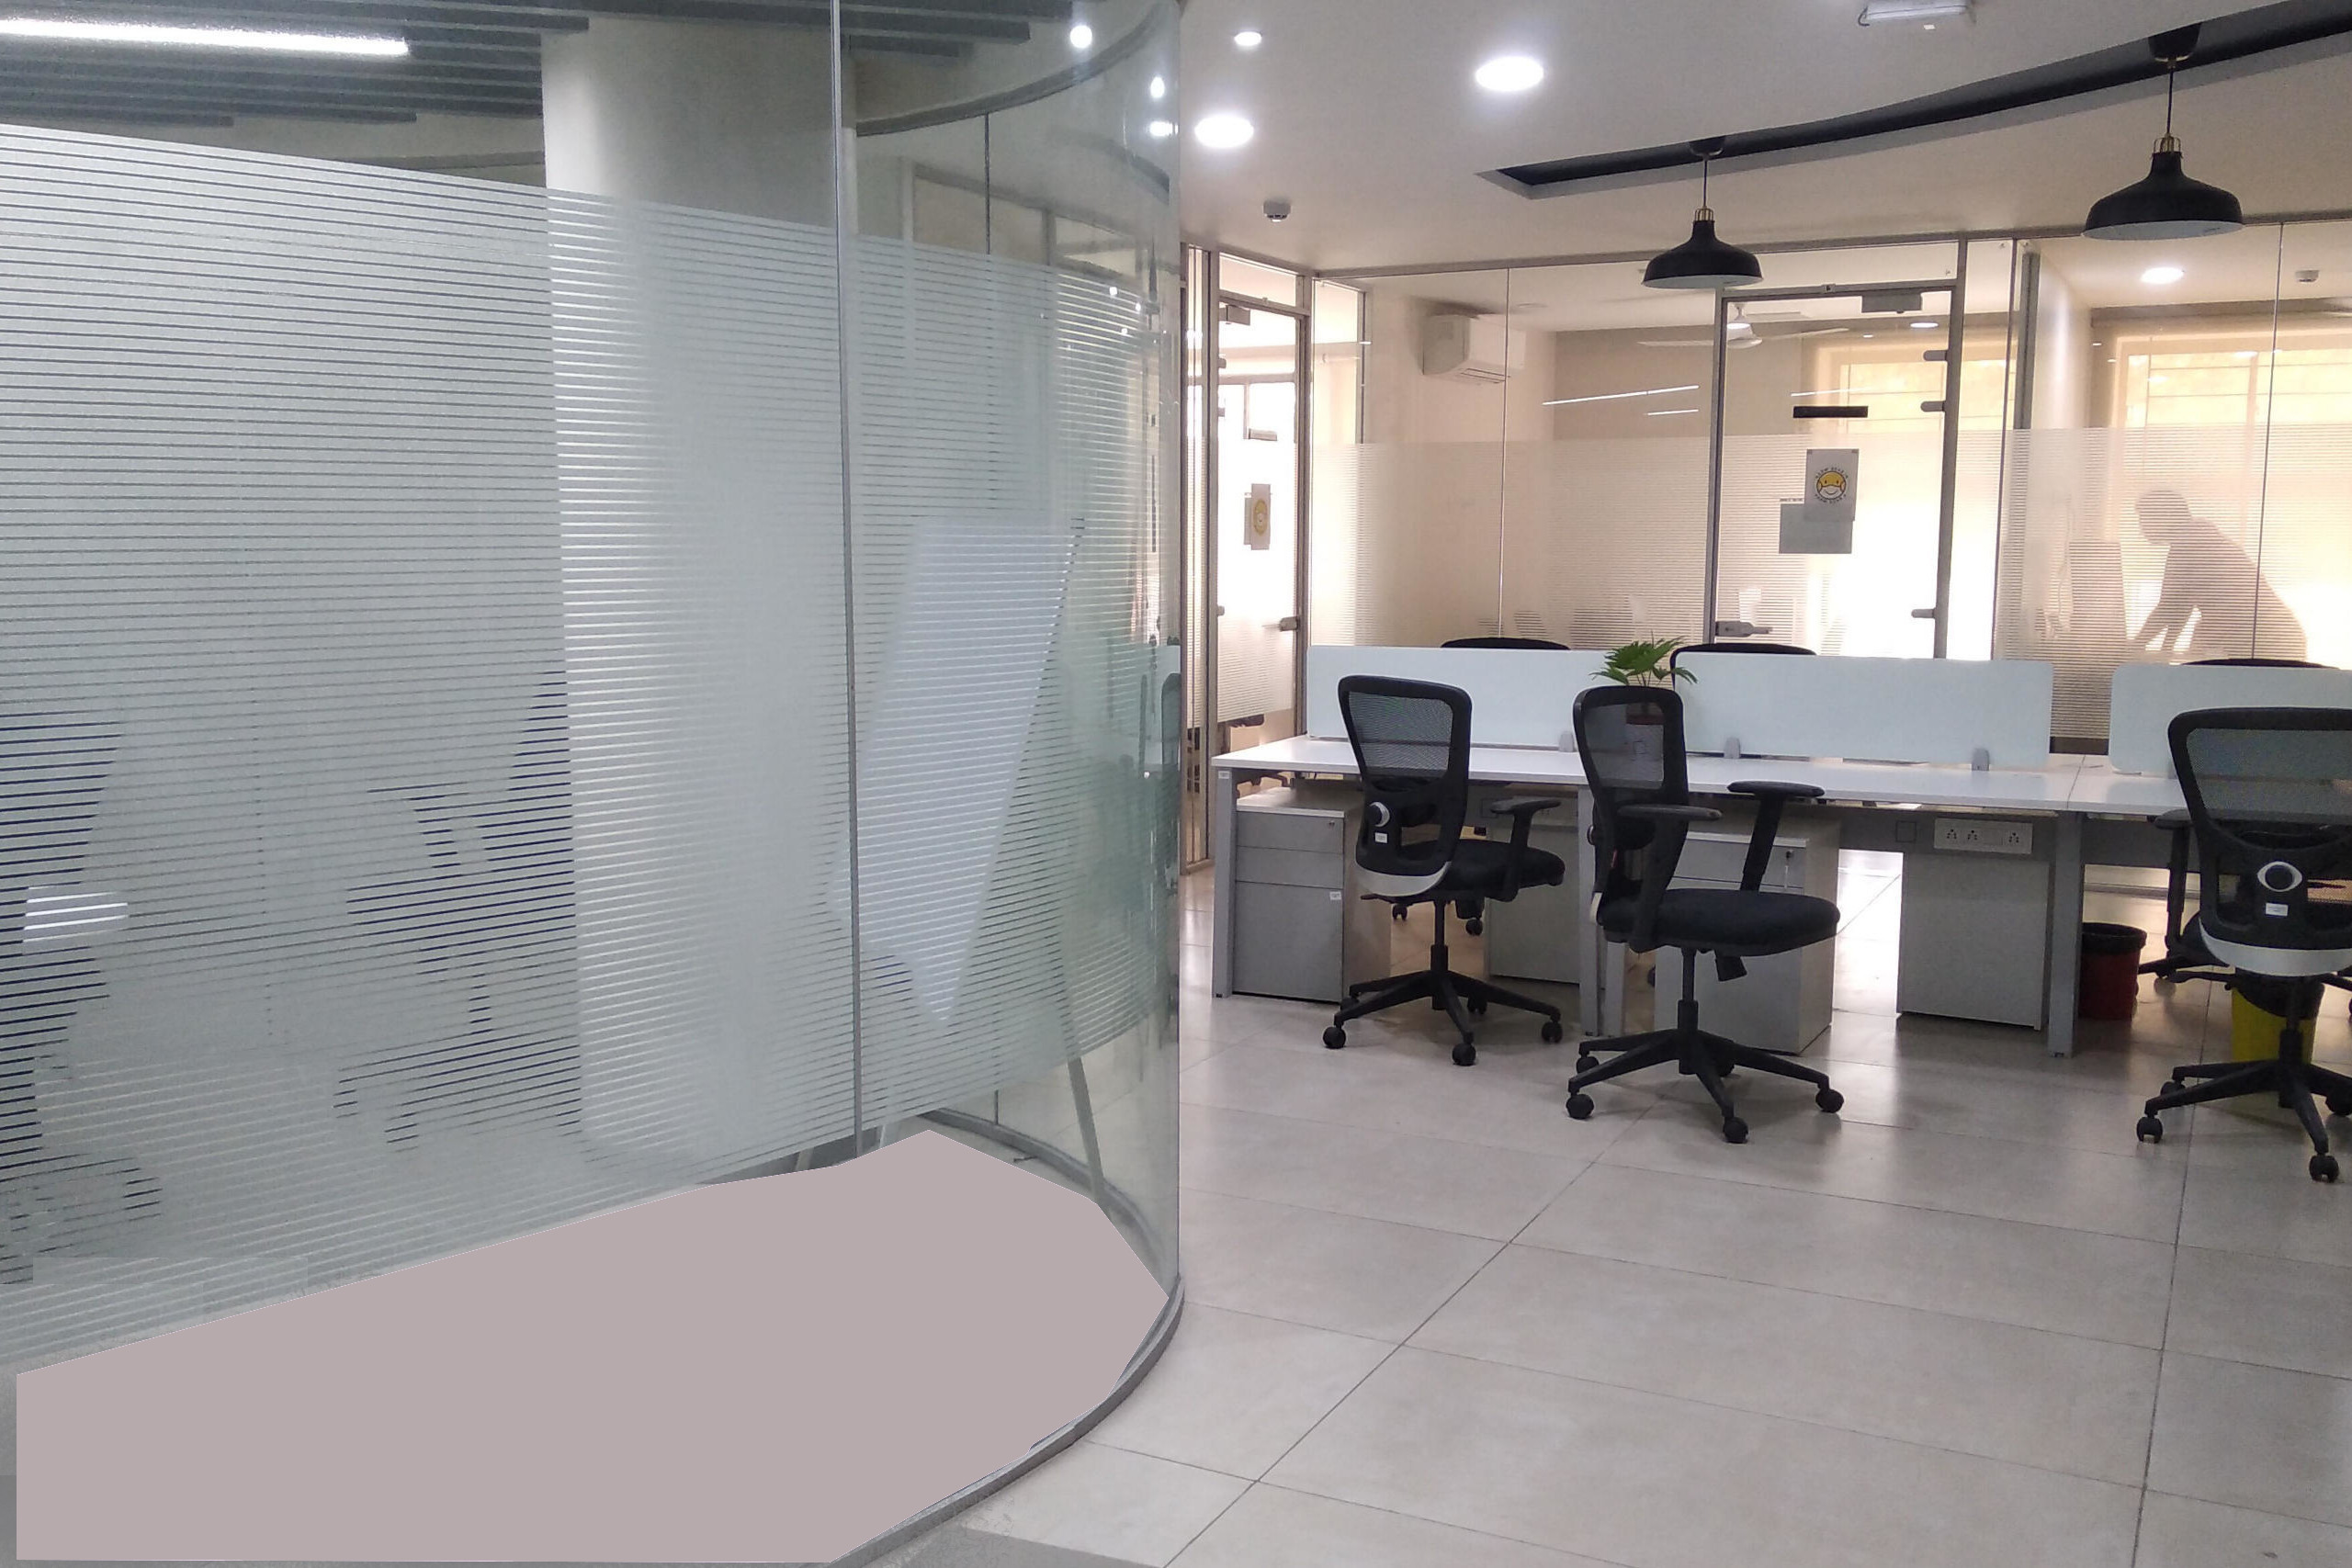
\includegraphics[height=\paperheight]{usach.jpg}}

\usetheme[sectionstyle=style3]{trigon}

% Definir los logotipos a utilizar (comentar si no hay logotipo)
\biglogo{usach_logo.jpg} % Se utiliza sólo en la portada
\smalllogo{_logo_small.png} % Se utiliza en la esquina superior derecha de los marcos normales

% ------ Si quieres cambiar los colores por defecto del tema, hazlo aquí ------
\definecolor{tPrim}{HTML}{eA0600}   % 716
\definecolor{tSec}{HTML}{3141B1}    % cool gray
\definecolor{tAccent}{HTML}{502F6C} % 294

 
% ------ Paquetes y definiciones utilizados para esta demostración. Se pueden eliminar ------
\usepackage{appendixnumberbeamer} % To use \appendix command
\pdfstringdefDisableCommands{% Fix hyperref translate warning with \appendix
\def\translate#1{#1}%
}
\usepackage{pgf-pie} % For pie charts 
\usepackage{caption} % For subfigures
\usepackage{subcaption} % For subfigures
\usepackage{xspace}
\newcommand{\themename}{\textbf{\textsc{USACHtheme}}\xspace}
\usepackage[scale=2]{ccicons} % Icons for CC-BY-SA
\usepackage{booktabs} % Better tables


%==============================================================================
%                               COMENZAR DOCUMENTO
%==============================================================================
\begin{document}

%--------------------------------------
% Create title frame
\titleframe

%--------------------------------------
% Table of contents
\begin{frame}{Overview}
  \setbeamertemplate{section in toc}[sections numbered]
  \tableofcontents[hideallsubsections]
\end{frame}


%==============================================
\section{Introduction}
%==============================================
\begin{frame}{\insertsectionhead}
  \framesubtitle{Outreach Programs}
  \textbf  On-campus and Off-campus programs
  \begin{itemize}
    \item 50-week Foundations of Modern Machine Learning - 250 intake (off-campus)
    \item 36-week Foundations of Modern Machine Learning - 180 intake (off-campus)
    \item 8-weeks paid Summer Research Internships - 100 intake (on-campus)
  \end{itemize}
\end{frame}


%==============================================
\section{50-week Foundations of Modern Machine Learning }
%==============================================

\subsection{Course Details}
\begin{frame}[fragile=singleslide]{\insertsectionhead}
  \framesubtitle{\insertsubsectionhead}
\begin{center}
\begin{itemize}
\item Chief Instructors - Prof CV Jawahar, Prof Anoop M, Dr Ravi Kiran 
\item Instructors - Wider pool of topic experts from IIIT Hyderabad
\item Live Interactive Session of 1.0 - 1.5 hrs duration per week
\item Distinguished Lectures - occasional
\item Distributed Personalised Tutorial Sessions - 20 per week
\item Weekly assignments, Monthly Projects and Quarterly Exams
\item Enrollment - 250 from all over India
\item Started in Oct 2021, Expected to end by July 2022
\end{itemize}
\end{center}
\end{frame}


%==============================================
\section{36-week Foundations of Modern Machine Learning }
%==============================================

\subsection{Course Details}
\begin{frame}[fragile=singleslide]{\insertsectionhead}
  \framesubtitle{\insertsubsectionhead}
\begin{center}
\begin{itemize}
\item Chief Instructors - Prof Anoop M, Dr Ravi Kiran 
\item Live Interactive Session of 1.0 - 1.5hrs duration per week
\item Distinguished Lectures - occasional
\item Distributed Personalised Tutorial Sessions - 20 per week
\item Weekly Assignments, Monthly Projects and Quarterly Exams
\item Enrollment - 180 from all over India
\item Started in Jan 2022, Expected to end by July 2022
\end{itemize}
\end{center}
\end{frame}


%==============================================
%\section{8-week Summer Research Internship}
%==============================================





%==============================================
\section{10th Edition of Workshop on Excitement of Research}
%==============================================

\subsection{Program Details}
\begin{frame}[fragile=singleslide]{\insertsectionhead}
  \framesubtitle{\insertsubsectionhead}
\begin{center}
\begin{itemize}
\item \textbf{Date : } Thursday, 21 April 2022
\item Invited Audience of over 650 - online Zoom
\item Inaugurated by Prof PJ Narayanan, Director IIIT Hyderabad
\item Prof CV Jawahar : IIIT Hyderabad
\item Anbumani Subramanian : Principal Research Engineer, Intel Inc
\item Prof U Deva Priyakumar : IIIT Hyderabad
\item Prof Syed Azeemuddin : IIIT Hyderabad
\end{itemize}
\end{center}
\end{frame}

%==============================================
\section{Ongoing Programs}
%==============================================

\subsection{Ongoing}

\begin{frame}[fragile=singleslide]{\insertsectionhead}
 % \framesubtitle{\insertsubsectionhead}
\begin{center}
\begin{itemize}
\item 50-week FMML commencing from August 2022
\item SRISHTI - 22
\item National Expo Data-Driven Solutions NEDDS-22
\begin{itemize}
\item Stakeholders from NM-ICPS - Govt, Academics, Industry, Start-ups, NGOs
\end{itemize}
\item Springer LNCS International Conference on BDA2022 (Big Data Analytics) 
\begin{itemize}
\item Co-organiser
\end{itemize}
\end{itemize}
\end{center}
\end{frame}

\subsection{\\50-week FMML - Aug 22}

\begin{frame}[fragile=singleslide]{\insertsectionhead - \insertsubsectionhead}
 % \framesubtitle{\insertsubsectionhead}
\begin{center}
\begin{itemize}
\item Based on learnings from prior FMML programs
\item Entry based on aptitude scores
\item Academic inclination - more homogeneous
\item Target - second year UG students only
\item Administer course modulewise -  one teacher per module
\item Hire permanent teachers/mentors - underway
\item DST confidence-building measure (large figures)
\end{itemize}
\end{center}
\end{frame}


\subsection{Program Details}
\begin{frame}[fragile=singleslide]{\insertsectionhead}
  \framesubtitle{\insertsubsectionhead}
\begin{center}
\begin{itemize}
\item Summer Internship Program at IIIT Hyderabad
\item \textbf{Period : } 16 May to 30 Jun
\item iHub funded Internship Program Rs 10,000 per student
\item Preliminary Selection from 7600+ (2650) students all over India
\item Admission Procedure - Exam (online + offline)
\item 126 students to work in thirteen Research Centres
\item 23 members of faculty currently supervising interns
\item Centralised training program (TNA) progressing simultaneously
\item 90 students listed to work remotely (unpaid)
\item \textbf{Waiting List : } Another 450 candidates, shared internally
\end{itemize}
\end{center}
\end{frame}


\subsection{\\SRISHTI 22}

\begin{frame}[fragile=singleslide]{\insertsectionhead - \insertsubsectionhead}
 % \framesubtitle{\insertsubsectionhead}
\begin{center}
\begin{itemize}
\item Goals, Objectives
\begin{itemize}
\item To imbibe a sense of academic and research inquiry to interns
\end{itemize}
\item Set expectations of interns
\begin{itemize}
\item Cognitive, General Skills, Personal 
\end{itemize}
\item Resources to interns
\begin{itemize}
\item Infrastructure, Compute
\end{itemize}
\item Success Metrics
\begin{itemize}
\item 40 percent of supervisors will re-appear next year
\item 20 percent of interns would publish a paper in a year
\item 10 percent of interns contribution would lead to product/patent in a year
\item 80 percent interns would report high satisfaction
\end{itemize}
\end{itemize}
\end{center}
\end{frame}

\subsection{\\SRISHTI 22}

\begin{frame}[fragile=singleslide]{\insertsectionhead - \insertsubsectionhead}
 % \framesubtitle{\insertsubsectionhead}
\begin{center}
\begin{itemize}
\item 11:30 am - 2:30 pm - Lectures/Tutorials/Special Sessions (all weekdays from 18 May to 24 June)
\item Progress Monitoring on Wednesdays - 18 May, 25  May, 01 June, 08 June, 15 June, 22 June	 
\end{itemize}
\end{center}
\end{frame}

\subsection{\\National-level Expo in November}

\begin{frame}[fragile=singleslide]{\insertsectionhead - \insertsubsectionhead}
 % \framesubtitle{\insertsubsectionhead}
\begin{center}
\begin{itemize}
\item C-DAC India agrees to be a partner 
\item Workshop on HPC on second day
\item Exploring options with Intel India
\end{itemize}
\end{center}
\end{frame}

%==============================================
\section{Fresh Plans}
%==============================================

\subsection{Outreach Activities}

\begin{frame}[fragile=singleslide]{\insertsectionhead}
  \framesubtitle{\insertsubsectionhead}
\begin{center}
\begin{itemize}
\item Scale Online Courses - Public Universities
\item Explore Long-term Online Internships - about to commence
\item Approach NIELIT for exploring joint online program
\item Joint Workshop bda2022.org Dec 19-22, 2022 at Hyderabad
\end{itemize}
\end{center}
\end{frame}



%-------------------------------------
%\end{document}
%--------------------------------------


\end{document}
